\chapter{Diseño e implementación} % Main chapter title

\label{Chapter3} % Change X to a consecutive number; for referencing this chapter elsewhere, use \ref{ChapterX}

\definecolor{mygreen}{rgb}{0,0.6,0}
\definecolor{mygray}{rgb}{0.5,0.5,0.5}
\definecolor{mymauve}{rgb}{0.58,0,0.82}

%%%%%%%%%%%%%%%%%%%%%%%%%%%%%%%%%%%%%%%%%%%%%%%%%%%%%%%%%%%%%%%%%%%%%%%%%%%%%
% parámetros para configurar el formato del código en los entornos lstlisting
%%%%%%%%%%%%%%%%%%%%%%%%%%%%%%%%%%%%%%%%%%%%%%%%%%%%%%%%%%%%%%%%%%%%%%%%%%%%%
\lstset{ %
  backgroundcolor=\color{white},   % choose the background color; you must add \usepackage{color} or \usepackage{xcolor}
  basicstyle=\footnotesize,        % the size of the fonts that are used for the code
  breakatwhitespace=false,         % sets if automatic breaks should only happen at whitespace
  breaklines=true,                 % sets automatic line breaking
  captionpos=b,                    % sets the caption-position to bottom
  commentstyle=\color{mygreen},    % comment style
  deletekeywords={...},            % if you want to delete keywords from the given language
  %escapeinside={\%*}{*)},          % if you want to add LaTeX within your code
  %extendedchars=true,              % lets you use non-ASCII characters; for 8-bits encodings only, does not work with UTF-8
  %frame=single,	                % adds a frame around the code
  keepspaces=true,                 % keeps spaces in text, useful for keeping indentation of code (possibly needs columns=flexible)
  keywordstyle=\color{blue},       % keyword style
  language=[ANSI]C,                % the language of the code
  %otherkeywords={*,...},           % if you want to add more keywords to the set
  numbers=left,                    % where to put the line-numbers; possible values are (none, left, right)
  numbersep=5pt,                   % how far the line-numbers are from the code
  numberstyle=\tiny\color{mygray}, % the style that is used for the line-numbers
  rulecolor=\color{black},         % if not set, the frame-color may be changed on line-breaks within not-black text (e.g. comments (green here))
  showspaces=false,                % show spaces everywhere adding particular underscores; it overrides 'showstringspaces'
  showstringspaces=false,          % underline spaces within strings only
  showtabs=false,                  % show tabs within strings adding particular underscores
  stepnumber=1,                    % the step between two line-numbers. If it's 1, each line will be numbered
  stringstyle=\color{mymauve},     % string literal style
  tabsize=2,	                   % sets default tabsize to 2 spaces
  title=\lstname,                  % show the filename of files included with \lstinputlisting; also try caption instead of title
  morecomment=[s]{/*}{*/}
}


%----------------------------------------------------------------------------------------

En este capítulo se explica el proceso que se siguió para desarrollar e implementar el prototipo de pruebas, el firmware, la interfaz web y el prototipo comercial.

%----------------------------------------------------------------------------------------

\section{Prototipo de pruebas}

El prototipo de pruebas fue desarrollado con la finalidad de probar todas las funciones de firmware que componen el trabajo, para brindar una primera aproximación al prototipo comercial del dispositivo.

Como se vio en el diagrama de la figura \ref{fig:diagramBlocks}, el dispositivo está compuesto por los siguientes bloques funcionales: microcontrolador, transceptor Wi-Fi, transceptor LoRa, memoria no volátil, reloj en tiempo real y conversor óptico-eléctrico.

La construcción del prototipo de pruebas se realizó en una \textit{breadboard}, que permitió realizar cambios en las conexiones de los componentes de una manera sencilla cuando estos se requerían. Se eligieron componentes de hardware acordes con los bloques que constituyen el dispositivo, en su mayor parte módulos de desarrollo con circuitos integrados embebidos que disponen de conectores apropiados para una breadboard. En la figura \ref{fig:blocksTest} se muestra el diagrama en bloques general con los componentes del prototipo de pruebas.

\begin{figure}[h]
	\centering
	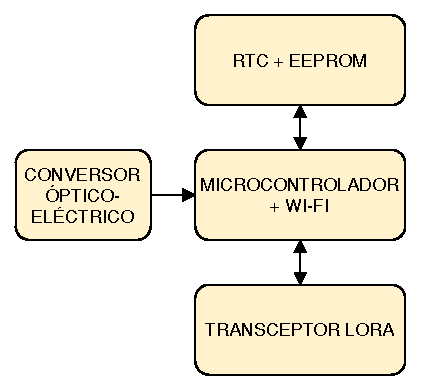
\includegraphics[scale=1]{./Figures/test_blocks.pdf}
	\caption{Diagrama en bloques del prototipo de pruebas.}
	\label{fig:blocksTest}
\end{figure}

Para garantizar un tiempo corto en la obtención de los componentes del prototipo de pruebas, el criterio predominante para la elección de los componentes fue la disponibilidad en el mercado local. Además, la elección de proveedores locales aseguró la restitución eficaz de los componentes que se malograron durante el desarrollo.

\subsection{Microcontrolador + Wi-Fi}

Este bloque fusiona los bloques microcontrolador y transceptor Wi-Fi. El desarrollo de dispositivos con conexión Wi-Fi ha tenido un gran crecimiento en los últimos años \citep{WEBSITE:19}, por lo que existen algunos fabricantes de circuitos integrados que ofrecen soluciones que integran microcontroladores y transceptores Wi-Fi en un solo encapsulado.

El componente elegido para este bloque es la tarjeta de desarrollo NodeMCU de la firma Amica, basado en el módulo ESP-12F de la firma Ai-Thinker. Las características más atractivas de esta tarjeta en lo referente al desarrollo son la alimentación y programación a través de un puerto micro USB, factor de forma adecuado para ser montado sobre un breadboard e incorporación de LEDs y pulsadores en la misma tarjeta. En la figura 3.2 se muestra la NodeMCU.

\begin{figure}[h]
	\centering
	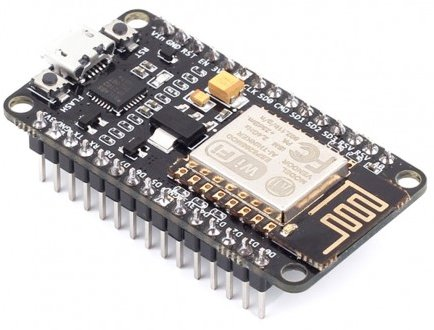
\includegraphics[scale=0.4]{./Figures/nodemcu.jpg}
	\caption{Tarjeta de desarrollo NodeMCU de la firma Amica\protect\footnotemark.}
		\label{fig:nodemcu}
	\end{figure}

	\footnotetext{Imagen tomada de: \url{https://www.amazon.com/-/es/KeeYees-Internet-Development-Wireless-Compatible/dp/B07PR9T5R5}}

El módulo ESP-12F monta sobre sí un SoC (\textit{System on a Chip}, sistema en un chip) de la firma Espressif Systems, el ESP8266, que funciona como microcontrolador y transceptor Wi.Fi. Otros componentes instalados sobre este módulo son condensadores, resistencias, oscilador, memoria flash y una antena impresa; todos ellos necesarios para que el ESP8266 pueda desempeñar correctamente sus funciones.

El ESP8266 es un chip de bajo costo que incorpora un microcontrolador y un transceptor Wi-Fi, además de contar con un \textit{stack} TCP/IP. Sus características técnicas más relevantes son:
\begin{itemize}
	\item Procesador Tensilica LX106 de arquitectura RISC (\textit{Reduced Instruction Set Computer}, computador con conjunto de instrucciones reducido) de 32 bits a una frecuencia de 80 MHz.
	\item RAM de 64 KB para instrucciones y 96 KB para datos.
	\item ROM externa, puede soportar hasta 16 MB de memoria flash con conexión QSPI (\textit{Quad} SPI, SPI cuádruple).
	\item IEEE 802.11 b/g/n.
	\item Periféricos GPIO (\textit{General Purpose Inputs/Outputs}, entradas/salidas de propósito general), SPI, I\textsuperscript{2}C, UART y ADC.
\end{itemize}

\subsection{Transceptor LoRa}

Para la elección del componente de este bloque hubo varias consideraciones. La más importante fue la frecuencia de transmisión y recepción. LoRa trabaja en las frecuencias de 433 MHz, 868 MHz y 915 MHz; de acuerdo al país donde se implementa. Esto en Bolivia el espectro electromagnético está normado por la Autoridad de Regulación y Fiscalización de Telecomunicaciones y Transportes, ATT, a través del documento de plan de frecuencias \citep{WEBSITE:17}. Allí se determina la frecuencia de 915 MHZ como la banda destinada para las aplicaciones ISM (\textit{Industrial, Scientific and Medical}; industrial científica y médica) que es usada en otros países para comunicaciones LoRa. Este tipo de comunicaciones no están contempladas en dicho documento, pero en el decreto supremo 4272 de fecha 24 de junio de 2020, en su artículo 73\citep{WEBSITE:27}, se especifica el procedimiento para la utilización de la frecuencia de 915 MHz para redes LPWAN (\textit{Low Power Wide Area Network}, redes de área amplia y bajo consumo) de manera libre.

En el mercado local no se pudieron encontrar módulos LoRa que funcionen a la frecuencia de 915 MHz. Se adquirieron los módulos disponibles, que trabajan en la frecuencia de 433 MHz, lo que según el plan de frecuencia boliviano \citep{WEBSITE:17} está destinado a radioaficionados. El módulo utilizado para el prototipo de pruebas fue el PM1280, que está basado el circuito integrado SX1278. En la figura \ref{fig:loraModule} se observa una fotografía del módulo PM1280.

\begin{figure}[h]
	\centering
	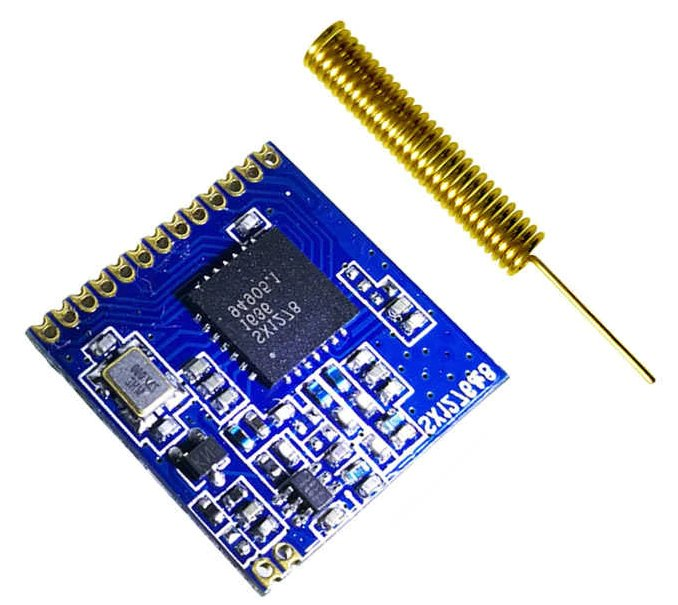
\includegraphics[scale=0.2]{./Figures/pm1280.jpg}
	\caption{Módulo LoRa PM1280\protect\footnotemark.}
		\label{fig:loraModule}
\end{figure}

\footnotetext{Imagen tomada de: \url{https://www.todomicro.com.ar/arduino/910-modulorf-lora-sx1278-chip-pm1280-con-antena.html}}

El circuito integrado SX1278 es un transceptor LoRa de la firma Semtech que provee comunicación de espectro ensanchado de largo alcance y alta inmunidad a las interferencias. Su principales características son:

\begin{itemize}
	\item Potencia de transmisión de 100 mW.
	\item Alta eficiencia del amplificador de potencia.
	\item Frecuencia de operación: 137 MHZ a 525 MHZ.
	\item Velocidad de bit programable hasta 300 Kbps.
	\item Bajo consumo de corriente, 9,9 mA en modo de recepción y 200 nA en la retención de datos en sus registros.
	\item Soporta paquetes de hasta 256 bytes.
	\item Sensor de temperatura e indicador de batería incorporados.
\end{itemize}


\subsection{RTC + EEPROM}

Los bloques memoria no volátil y reloj en tiempo real fueron fusionados en un único bloque, ya que comercialmente existen módulos que cumplen ambas funciones. Estos módulos tienen embebidos circuitos integrados de memoria y RTC, además de otros componentes como resistencias, condensadores, osciladores, zócalos para baterías y conectores apropiados para un breadboard. Estos módulos en su gran mayoría poseen una EEPROM como medio de almacenamiento de datos, esta tecnología es preferible sobre las memorias flash en aplicaciones de adquisición de datos, ya que proporciona un número mayor de ciclos de escritura y borrado.

La mayor parte de los módulos que existen en el mercado local cumplen cabalmente con las funciones que requiere este bloque, pero debido a la cantidad de pines utilizables de la NodeMCU se tuvo preferencia por los módulos que tenían integrados chips con interfaz I\textsuperscript{2}C. Asimismo, al haber muchos módulos que cumplían el requisito de la interfaz, se buscó uno que tuviera un RTC con la capacidad de generar alarmas en función de la hora. En la figura 3.2 se observa el módulo de RTC + EEPROM elegido.

\begin{figure}[h]
	\centering
	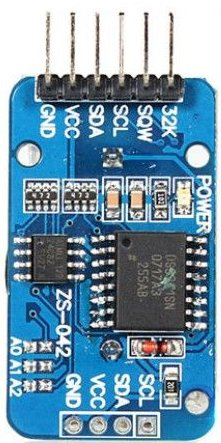
\includegraphics[scale=0.35]{./Figures/rtc_eeprom.jpg}
	\caption{Módulo RTC + EEPROM\protect\footnotemark.}
		\label{fig:cuadradoAzul}
	\end{figure}

	\footnotetext{Imagen tomada de: \url{https://electropeak.com/extremely-accurate-rtc-module}}

Los circuitos integrados que componen el módulo son el DS3231 y el AT24C32, un RTC y una EEPROM, respectivamente. El DS3231 es un RTC de alta precisión de la firma Maxim Integrated, que cuenta con una interfaz I\textsuperscript{2}C para conectarse con otros dispositivos, también tiene la capacidad de generar alarmas y medir la temperatura. El AT24C32 es una EEPROM de la firma Microchip, con interfaz I\textsuperscript{2}C y 32 KB de capacidad de almacenamiento.

\subsection{Conversor óptico-eléctrico}

Para este bloque, el componente elegido es un módulo detector de luz, compuesto por un fototransistor PT333-3C de la firma Everlight y un comparador de voltaje LM393 de la firma Texas Instruments. El módulo genera como salida un pulso eléctrico acotado al nivel de tensión con el que se alimenta. Cuando la cantidad de luz incidente en el fototransistor provoca un nivel de tensión igual o mayor al nivel de tensión del potenciómetro que viene incluido. En la figura \ref{fig:coeModule} se puede observar el módulo.

\begin{figure}[h]
	\centering
	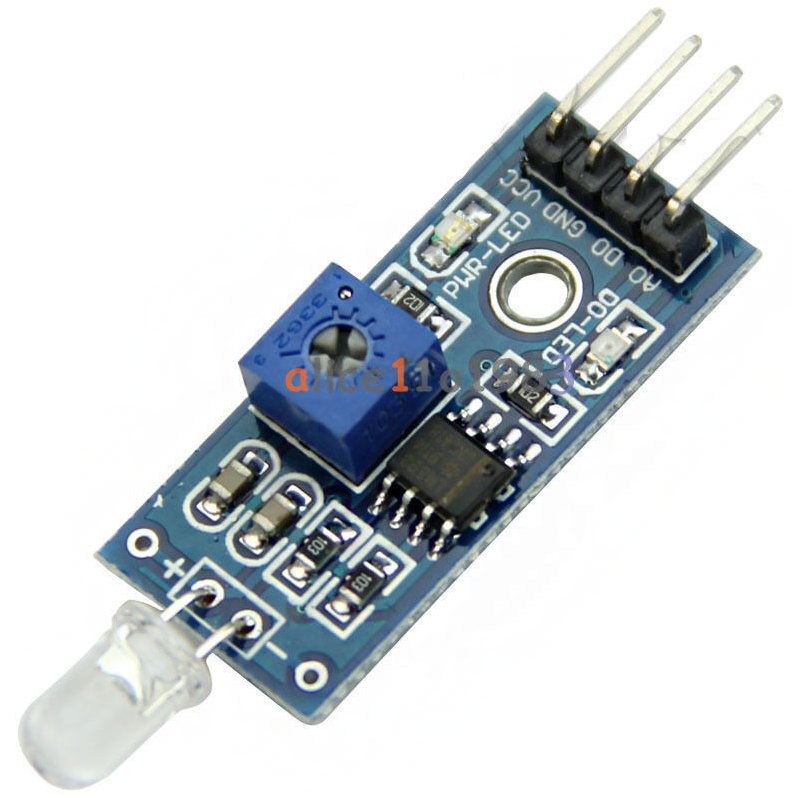
\includegraphics[scale=0.2]{./Figures/coe.jpg}
	\caption{Módulo detector de luz\protect\footnotemark.}
		\label{fig:coeModule}
\end{figure}

	\footnotetext{Imagen tomada de: \url{https://www.roboter-bausatz.de/en/diy-electronics/extension-modules/sensors/optics-light/149/light-sensor-module}}

%----------------------------------------------------------------------------------------

\section{Diseño de firmware}

El desarrollo del firmware fue la actividad que requirió más esfuerzo en el trabajo, debido a que el principal objetivo del autor fue escribir código que pudiera ser reutilizado en futuros proyectos. Otro objetivo fue lograr modularización en el código escrito, que permitiera probar cada módulo de firmware individualmente. Para lograr dichos objetivos, el firmware fue estructurado en capas y se utilizó control de versiones para documentarlo. De esta manera, se logró un desarrollo de carácter más profesional que podría ser reutilizado en futuros proyectos que requieran funciones similares.

Antes de realizar la separación del firmware en capas, fue necesario elegir las herramientas de desarrollo implicadas, que fueron imprescindibles al momento de escribir el código fuente del dispositivo. Estas herramientas fueron un SDK (\textit{Software Deveplopment Kit}, kit de desarrollo de software) que proporcionó una API (\textit{Application Programming Interface}, interfaz de programación de aplicaciones) para facilitar el desarrollo de código fuente para el ESP8266 y un IDE (\textit{Integrated Development Enviroment}, Entorno de Desarrollo Integrado) que proporcionó un entorno con herramientas que agilizaron la escritura de código con el SDK elegido. Estos fueron:

\begin{itemize}
	\item ESP8266\_RTOS\_SDK: este SDK fue desarrollado por la firma Espressif Systems para la programación del SoC ESP8266 y facilita un conjunto de funciones para la creación de código fuente. Está basado en el RTOS (\textit{Real-Time Operating System}, sistema operativo en tiempo real) de uso gratuito FreeRTOS \citep{WEBSITE:18}, que fue utilizado en las materias sobre sistemas operativos en tiempo real de la Carrera de Especialización y brindó funciones que ayudaron a lograr determinismo en la ejecución de las tareas del dispositivo. Asimismo, contiene un documentación completa sobre las funciones que incorpora y ejemplos de uso.
	\item Eclipse: el aspecto más importante en la elección de este IDE fue que en la documentación de instalación y uso del ESP8266\_RTOS\_SDK \citep{WEBSITE:23}, se indicaba el proceso de configuración que permitió utilizar ambos en conjunto. Otro aspecto de importancia fue la experiencia previa del autor con este IDE, fue utilizado en varias materias de la Carrera de Especialización.
\end{itemize}

Entonces, una vez definidas las herramientas utilizadas, fue posible dividir el firmware en capas para facilitar el desarrollo y reducir la complejidad del código escrito para el dispositivo. La división en capas del firmware puede observarse en el diagrama de la figura \ref{fig:firmwareLayers}, donde existen tres capas claramente diferenciadas: APP, DRIVERS y BASE.

\begin{figure}[h]
	\centering
	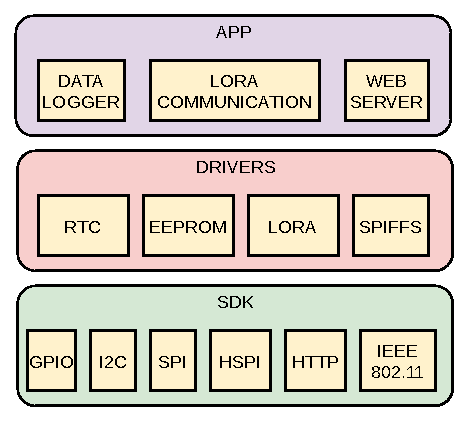
\includegraphics[scale=1]{./Figures/firmware_layers.pdf}
	\caption{Diagrama de capas del firmware.}
		\label{fig:firmwareLayers}
\end{figure}

BASE es la capa de menor nivel y está compuesta por la API del ESP8266\_RTOS\_SDK. Proporciona a las capas de niveles superiores la capacidad de interactuar con los periféricos y protocolos del ESP8266 a través de funciones en lenguaje C. Los periféricos y protocolos que fueron utilizados en el presente trabajo fueron:

\begin{itemize}
	\item GPIO: este periférico fue utilizado por la capa APP para gestionar los pines disponibles en el ESP8266, ya que algunos de ellos tienen funciones específicas y no pueden ser utilizados para propósitos generales. La API posee funciones para definir los pines como entradas o salidas, configuración de interrupciones por flanco positivo o negativo y resistencias de \textit{pull-up} internas.
	\item I\textsuperscript{2}C: se utilizó este periférico para que la capa DRIVERS interactúe con el RTC y la EEPROM. Al tener pocos pines disponibles en el ESP8266, este componente se hizo muy importante, ya que la comunicación I\textsuperscript{2}C solo requiere dos pines, uno para datos y otro el reloj de sincronización.
	\item SPI: la capa DRIVERS utiliza este periférico para comunicarse con el transceptor LoRa. El módulo LoRa elegido interacciona a través del protocolo SPI con el microcontrolador que lo maneja para transmitir o recibir datos.
	\item HSPI: el ESP8266 no posee memoria ROM embebida en el SoC, por tanto, utiliza una memoria flash externa para almacenar las instrucciones del programa y los datos del usuario. Esta memoria flash se comunica con el ESP8266 mediante el protocolo HSPI. Este periférico se utilizó para que la capa DRIVERS configure la flash como un sistema de archivos.
	\item HTTP (\textit{HyperText Transfer Protocol}, protocolo de transferencia de hipertexto): la API ofrece funciones para ejecutar este protocolo. Fue de utilidad para proporcionar a la capa APP las funciones necesarias para implementar un servidor web capaz de responder a los métodos HTTP, GET y POST \citep{WEBSITE:20}.
	\item IEEE 802.11: el ESP8266 tiene embebida toda la electrónica necesaria para implementar los protocolos IEEE 802.11 en sus versiones b, g y n. La capa APP utilizó las funciones disponibles de este módulo para lograr que el dispositivo funcionara como punto de acceso y/o estación.
\end{itemize}

La capa DRIVERS está compuesta por módulos que son bibliotecas de firmware, que le permiten al ESP8266 interactuar con los periféricos de hardware externos a los que está conectado. Se desarrollaron bibliotecas para los módulos EEPROM, RTC, LORA y SPIFFS; todos basados en la capa BASE. Estas bibliotecas se encuentran en el repositorio del trabajo y constan de un archivo de código fuente y otro de cabecera, cada una.

La biblioteca para la EEPROM se desarrolló con ayuda del \textit{datasheet} \citep{WEBSITE:24} del AT24C32, donde se indican todos los pormenores técnicos del funcionamiento de este circuito integrado. Además, se utilizaron las funciones de la capa BASE para gestionar correctamente la comunicación I\textsuperscript{2}C. Las funciones que proporciona esta biblioteca sirven para:

\begin{itemize}
	\item leer de valores de 8, 16 y 32 bits de una dirección determinada de la EPROM.
	\item escribir de valores de 8, 16 y 32 bits de una dirección determinada de la EPROM.
\end{itemize}

Para el módulo RTC se desarrolló una biblioteca que sirvió para configurar la hora, fecha y otras funciones incorporadas en el DS3231. La herramienta principal en el desarrollo de esta biblioteca fue el datasheet \citep{WEBSITE:25} de dicho circuito integrado. De este se obtuvo información sobre las direcciones de los registros que manejan sus funciones y la forma adecuada de configurarlos. Igual que para la biblioteca de la EEPROM, las funciones de la capa BASE para el protocolo I\textsuperscript{2}C permitieron que se disponga de una manera para que el ESP8266 pueda intercambiar datos con el DS3231 con la menor cantidad de pines posible. Esta biblioteca permite:

\begin{itemize}
	\item leer y configurar las horas, minutos y segundos.
	\item leer y configurar el día, fecha, mes y año.
	\item leer y configurar las dos alarmas disponibles.
	\item leer y configurar las salidas digitales.
	
\end{itemize} 

El desarrollo de la biblioteca para el módulo LORA permitió manejar el circuito integrado SX1278, para establecer la comunicación de este elemento con el ESP8266 a través del periférico SPI. Esto permitió configurar sus parámetros para lograr la transmisión y recepción de datos con dispositivos de tecnología LoRa de manera exitosa. Está basada en la biblioteca Arduino LoRa de Sandeep Mistry \citep{WEBSITE:21} y en la información del datasheet \citep{WEBSITE:26} del SX1278. Asimismo, utiliza las funciones proporcionadas por la capa BASE para la comunicación SPI. Las funciones más importantes que proporciona son:

\begin{itemize}
	\item configurar la frecuencia del módulo.
	\item transmitir un \textit{buffer} de tamaño variable.
	\item recibir datos en el buffer interno.
	\item leer el valor del RSSI (\textit{Received Signal Strength Indication}, indicador de fuerza de la señal recibida) de los datos recibidos en el buffer interno.
	\item establecer el modo de funcionamiento en bajo consumo.
	\item configurar la potencia de transmisión.
	\item configurar el ancho de banda.
	\item habilitar/deshabilitar el CRC (\textit{Cyclic Redundancy Check}, verificación de redundancia cíclica).
\end{itemize}

Por último, se desarrolló una biblioteca para establecer un sistema de archivos muy reducido llamado SPIFFS (SPI \textit{Flash File System}, sistema de archivos flash SPI), que está albergado en la memoria flash externa utilizada para almacenar el programa del ESP8266. Esta biblioteca requirió menos esfuerzo en su desarrollo que las anteriores, debido a que la mayoría de las funciones necesarias para configurar el sistema de archivos son parte de la API del ESP8266\_RTOS\_SDK y para el manejo de archivos se utilizaron las funciones estándar de C. Solo posee una función para inicializar el sistema de archivos, que configura la cantidad máxima de elementos y su capacidad de almacenamiento.

El tamaño de este sistema de archivos es de 1 MB y fue configurado de acuerdo al tamaño total de la memoria flash, que en el módulo ESP-12F es de 4 MB. El restante se utilizó para el programa, datos de fábrica y datos de configuración de la interfaz física. El detalle de los archivos almacenados en SPIFFS puede observarse en la tabla \ref{tab:spiffsDetail}.

\begin{table}[h]
	\centering
	\caption[Contenido SPIFFS]{Tabla de detalle del contenido del sistema de archivos SPIFFS.}
	\begin{tabular}{l c c}    
		\toprule
		\textbf{Nombre} & \textbf{Tamaño (KB)} & \textbf{Descripción} \\
		\midrule
		ajax-loadergif.gif & 6,2 & Imagen de carga de la interfaz web \\
		favicon.ico & 1,1 & Ícono de la interfaz web\\
		highchartsjs.gz	& 92 & Biblioteca JavaScript Highcharts comprimida \\
		highchartsmap.gz & 235,6 & Archivo de mapeo para highchartsjs.gz \\
		index.html & 7,3 & Documento HTML de la interfaz web \\
		jqueryjs.gz & 33,2 & Biblioteca JavaScript jQuery comprimida \\
		jquerymobilecss.gz & 25,1 & Hoja de estilos CSS de la bibliote jQuery Mobile \\
		jquerymobilejs.gz & 55,5 & Biblioteca JavaScript jQuery Mobile comprimida \\
		jquerymobilemap.gz & 88,8 & Archivo de mapeo para jquerymobilejs.gz \\
		config.txt & 0,6 & Archivo de configuración del dispositivo \\
		pulses.csv & 1 & Archivo con el registro histórico del consumo eléctrico \\
		
		\bottomrule
		\hline
	\end{tabular}
	\label{tab:spiffsDetail}
\end{table}

La mayoría de los archivos almacenados en SPIFFS son utilizados para generar la interfaz web, excepto config.txt y pulses.csv. El tamaño de memoria utilizado por todos los archivos es de 546,4 KB, que ocupa aproximadamente un 54\% del tamaño total del sistema de archivos. Hay que notar que los archivos de mayor tamaño fueron comprimidos antes de ser almacenados, ya que sin este proceso el tamaño total hubiera sido de 1,6 MB, que superaba aproximadamente en un 60\% el tamaño del sistema de archivos.

La capa APP, está compuesta por los módulos que ejecutan las tareas del dispositivo. Se basa en las capas inferiores para interactuar con los periféricos del ESP8266 y con el hardware externo. Sus módulos son DATA LOGGER, DATA COMMUNICATION y WEB SERVER. Los archivos de estos módulos se encuentran en el repositorio del trabajo.

\subsection{DATA LOGGER}

Este módulo tiene la función principal de adquirir, procesar y almacenar la información de consumo eléctrico del medidor al que está instalado el dispositivo. Para este fin, se comunica con los módulos de las capas inferiores como se muestra en el diagrama de la figura \ref{fig:dataLayers}.

\begin{figure}[h]
	\centering
	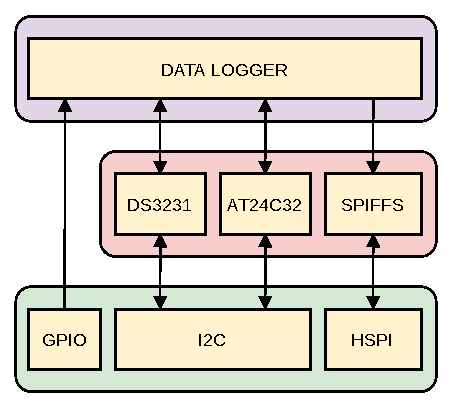
\includegraphics[scale=1]{./Figures/data_logger_diagram.pdf}
	\caption{Diagrama de capas para DATA LOGGER.}
		\label{fig:dataLayers}
\end{figure}

Utiliza el RTC y la EEPROM para mantener un registro histórico de la información adquirida por GPIO. Modifica el archivo pulses.csv almacenado en SPIFFS para actualizar la información de consumo eléctrico cuando se registran nuevos datos. Esto es utilizado posteriormente por WEB SERVER. Asimismo, en función de las alarmas generadas por el RTC, se envían los datos de la EEPROM a DATA COMMUNICATION.

Dentro del sistema operativo utilizado existen dos tareas para este módulo. Una para registrar los pulsos del medidor eléctrico y otra para manejar las alarmas del RTC, pulses\_task y alarm\_task. Estas tareas utilizaron algunas herramientas proporcionadas por FreeRTOS para gestionar la comunicación de los módulos. En la figura \ref{fig:dataRTOS} se observa un diagrama que muestra la manera en que se realiza la comunicación con ayuda de las herramientas de FreeRTOS.

\begin{figure}[h]
	\centering
	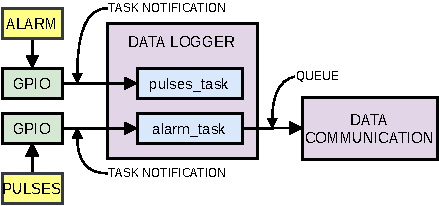
\includegraphics[scale=1]{./Figures/data_logger_com.pdf}
	\caption{Diagrama de conexión con las herramientas de FreeRTOS de DATA LOGGER.}
		\label{fig:dataRTOS}
\end{figure}

De la figura \ref{fig:dataRTOS}, ALARM representa las alarmas generadas por el RTC y PULSES los pulsos eléctricos provenientes del conversor óptico-eléctrico. PULSES y ALARM son conectados cada uno a un pin manejado por GPIO, que utiliza interrupciones por flanco de subida para generar notificaciones a pulses\_task y alarm\_task. Una de las funciones de la tarea alarm\_task es enviar por una cola los datos de consumo eléctrico a DATA COMMUNICATION.  Mediante los diagramas de flujo de las figuras \ref{fig:flowDataPulses} y \ref{fig:flowDataAlarm}, se puede apreciar el funcionamiento de estas tareas.

\begin{figure}[h]
	\centering
	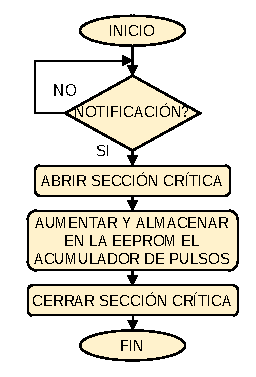
\includegraphics[scale=0.91]{./Figures/data_logger_pulses.pdf}
	\caption{Diagrama de flujo de la tarea pulses\_task.}
		\label{fig:flowDataPulses}
\end{figure}

\begin{figure}[h]
	\centering
	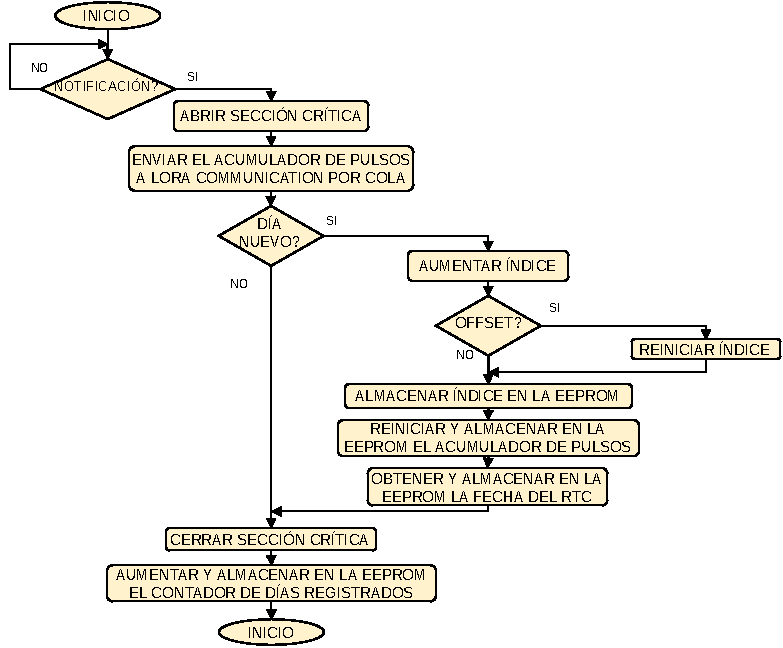
\includegraphics[scale=0.91]{./Figures/data_logger_alarm.pdf}
	\caption{Diagrama de flujo de la tarea alarm\_task.}
		\label{fig:flowDataAlarm}
\end{figure}

Según el diagrama de flujo de la figura \ref{fig:flowDataPulses}, la tarea pulses\_task espera por una notificación provocada por el flanco de subida de los pulsos eléctricos del conversor óptico-eléctrico. Cuando esto ocurre, se abre una sección crítica para prevenir que existan cambios de contexto dentro del sistema operativo que modifiquen los datos implicados antes de que estos puedan ser utilizados. Una vez en la sección crítica, en una variable de 16 bits se acumulan la cantidad de pulsos detectados y se almacenan en la EEPROM, en una dirección de memoria definida por una variable que hace referencia al índice. Finalmente, se cierra la sección crítica y este proceso se lleva a cabo mientras el dispositivo funcione. Esta es la función más importante del dispositivo, por lo que se le dedicó mayor tiempo y esfuerzo.

En el diagrama de la figura \ref{fig:flowDataAlarm}, los pulsos eléctricos generados por el RTC crean una notificación a la tarea alarm\_task. Si se detecta una notificación, se abre una sección crítica donde mediante una cola se envía el valor de la variable acumuladora de pulsos al módulo DATA COMMUNICATION. Con ayuda del RTC, si se detecta un cambio de fecha, se ejecutan instrucciones para que la cantidad de pulsos contada a partir de ese momento se reinicie y se almacene en un posición diferente de la EEPROM, lo que evita que los datos en esta memoria se sobrescriban mientras exista espacio suficiente para almacenar más información. Si no se detecta un cambio en la fecha o en caso contrario, se ejecutó todo el proceso antes descrito para la modificación del índice de la EEPROM, la tarea termina, pero vuelve a repetirse cada vez que ocurre una nueva notificación.

Para que este módulo funcione correctamente cuando el dispositivo es encendido se ejecuta una función de inicialización. En el diagrama de flujo de la figura \ref{fig:flowDataInit} se ilustra su comportamiento.

\begin{figure}[h]
	\centering
	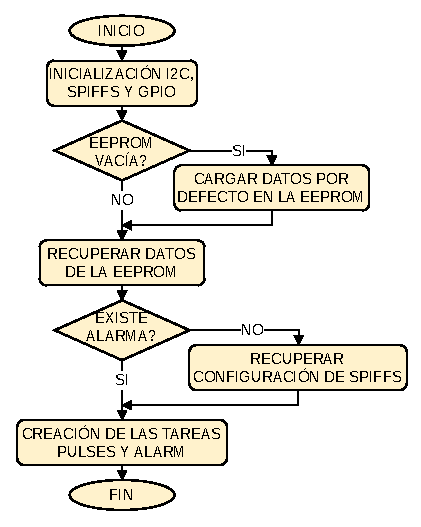
\includegraphics[scale=1]{./Figures/data_logger_init.pdf}
	\caption{Diagrama de flujo de la función de inicialización de DATA LOGGER.}
		\label{fig:flowDataInit}
\end{figure}

El procedimiento de inicialización del módulo, empieza con la configuración de los periféricos I\textsuperscript{2}C y GPIO para utilizar sus funciones. También se inicializa el sistema de archivos SPIFFS para tener la capacidad de leer y modificar todos los elementos almacenados. Se hace una lectura de la EEPROM para verificar si esta tiene datos de un funcionamiento anterior y en caso positivo almacenar los datos por defecto. Se recuperan los datos previamente cargados y se configura la alarma del RTC con los datos obtenidos del archivo config.txt almacenado en SPIFFS. Finalmente, se crean las tareas pulses\_task y alarm\_task.

\subsection{DATA COMMUNICATION}	

La función de este módulo se basa en utilizar el transceptor LoRa para intercambiar información con un dispositivo concentrador de datos de la misma tecnología. Sus tareas principales son enviar la cantidad de pulsos registrados y recibir parámetros de funcionamiento. Para esto, se comunica con otros módulos de las capas inferiores como se muestra en la figura \ref{fig:loraDiagram}.

\begin{figure}[h]
	\centering
	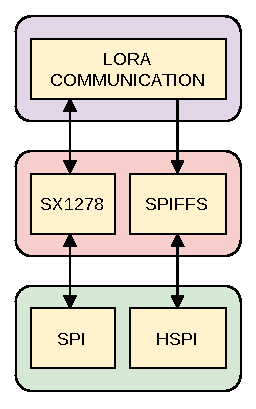
\includegraphics[scale=1]{./Figures/lora_communication_diagram.pdf}
	\caption{Diagrama de capas para LORA COMMUNICATION.}
		\label{fig:loraDiagram}
\end{figure}

Para que este módulo pueda enviar o recibir información utiliza las funciones proporcionadas por LORA, que a su vez utiliza el periférico SPI, para conmutar el modo de operación. Cuando recibe información del dispositivo concentrador de datos se accede a SPIFFS para modificar el archivo config.txt, lo que actualiza los parámetros de funcionamiento del dispositivo.

Este módulo posee una solo tarea que se ejecuta en el sistema operativo, nombrada lora\_task. En la figura \ref{fig:loraTask} puede observarse su comportamiento mediante un diagrama de flujo.

\begin{figure}[h]
	\centering
	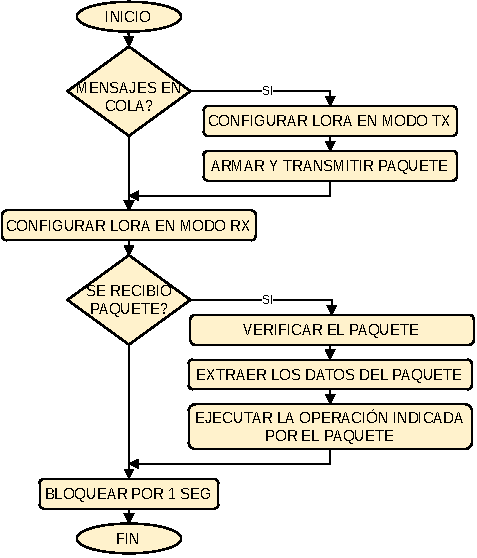
\includegraphics[scale=1]{./Figures/lora_communication_task.pdf}
	\caption{Diagrama de flujo de la tarea lora\_task.}
		\label{fig:loraTask}
\end{figure}

Del diagrama de la figura \ref{fig:loraTask}, esta tarea consulta la cola de mensajes para determinar si existe algún elemento pendiente de atención. Si existen mensajes pendientes en la cola se configura el transceptor LoRa en modo de transmisión, se arma un paquete con la información necesaria y se envía. Si la cola está vacía o se envió un paquete anteriormente, se configura el transceptor LoRa en modo de recepción y cuando se recibe un paquete se ejecuta la acción requerida por este. Finalizado todo este proceso la tarea se bloquea por un segundo y vuelve a repetirse mientras el dispositivo esté en funcionamiento.

El formato de los paquetes es el que se muestra en la figura \ref{fig:loraRxPacket}. Donde SRC es un campo de 8 Bytes, identificador de la fuente del paquete. DEST tiene una longitud de 4 Bytes e indica el destinatario del paquete. OP es de 1 Byte y define las operaciones solicitadas al dispositivo, que pueden ser la modificación del archivo config.txt, configuración de la hora y fecha, solicitud de los datos de la EEPROM, por citar algunas. PARAM1 y PARAM2 son campos de 32 Bytes cada uno, contienen los parámetros con los que se deben ejecutar las operaciones requeridas por el campo OP.

\begin{figure}[h]
	\centering
	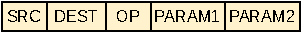
\includegraphics[scale=1]{./Figures/lora_communication_rx_packet.pdf}
	\caption{Formato de los paquetes enviados y recibidos por DATA COMMUNICATION.}
		\label{fig:loraRxPacket}
\end{figure}

Este módulo tiene una función de inicialización que debe ser ejecutada cuando el dispositivo es energizado y el ESP8266 empieza a ejecutar el código que tiene grabado. Su comportamiento se muestra en el diagrama de flujo presentado en la figura \ref{fig:loraInit}

\begin{figure}[h]
	\centering
	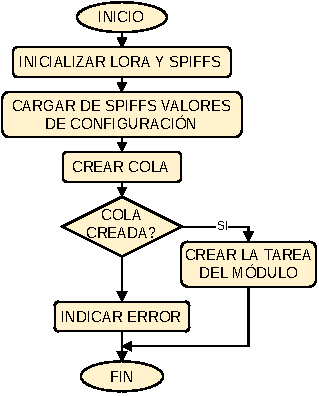
\includegraphics[scale=1]{./Figures/lora_communication_init.pdf}
	\caption{Diagrama de flujo de la función de inicialización del módulo LORA COMMUNICATION.}
		\label{fig:loraInit}
\end{figure}

Esta función de inicialización ejecuta todos los procesos necesarios para configurar el transceptor LoRa antes de utilizarlo. Posteriormente, intenta crear una cola para recibir información del módulo DATA LOGGER. Si esta no puede ser creada termina la función e indica un error. Finalmente, si el proceso anterior se realizó exitosamente se crea la tarea lora\_tasl que deberá ejecutarse para transmitir y recibir paquetes durante el funcionamiento del dispositivo. 

\subsection{WEB SERVER}

El objetivo de este módulo es establecer un servidor web con la capacidad de conectarse con dispositivos que dispongan de conexión Wi-Fi, para permitirles leer o modificar lo contenido del sistema de archivos. Para cumplir con lo planteado anteriormente, se utilizan los componentes de las capas inferiores como indica la figura \ref{fig:serverDiagram}.

\begin{figure}[h]
	\centering
	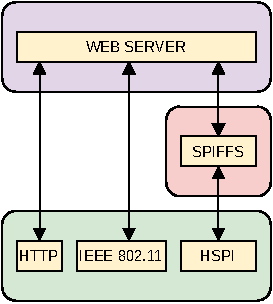
\includegraphics[scale=1]{./Figures/web_server_diagram.pdf}
	\caption{Diagrama de capas para WEB SERVER.}
		\label{fig:serverDiagram}
\end{figure}

WEB SERVER utiliza las funciones del protocolo HTTP para establecer un servidor que puede comunicarse con múltiples clientes HTTP mediante los métodos GET y POST, para la transferencia y modificación de los archivos almacenados en SPIFFS. El módulo IEEE 802.11 proporciona funciones para que WEB SERVER configure todas las funciones disponibles del transceptor Wi-Fi del ESP8266.

Este módulo puede configurar el dispositivo como punto de acceso o como estación. Esto se hace de manera automática y depende de la información contenida en el archivo de configuración almacenado en SPIFFS, config.txt. Si existe información de red, el dispositivo se configura como estación, en caso contrario, como punto de acceso. En cualquiera de los dos modos citados los clientes pueden acceder al servidor a través de su dirección de red como indican las figuras \ref{fig:serverAP} y \ref{fig:serverSTA}.                                                                                                                                                                                                                                                                                                                                                                                                                                                                                                                                                                                                                                                                                                                                                                                                                                                                                                                                                                                                                                                                          

\begin{figure}[h]
	\centering
	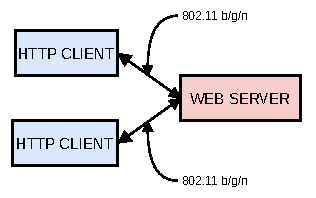
\includegraphics[scale=1.1]{./Figures/web_server_ap.pdf}
	\caption{WEB SERVER en modo punto de acceso.}
		\label{fig:serverAP}
\end{figure}

\begin{figure}[h]
	\centering
	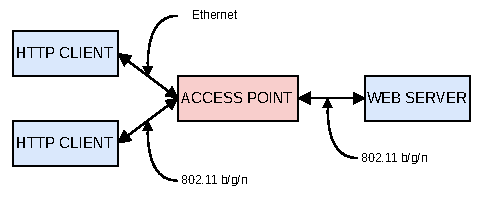
\includegraphics[scale=1.1]{./Figures/web_server_sta.pdf}
	\caption{WEB SERVER en modo estación.}
		\label{fig:serverSTA}
\end{figure}

En la figura \ref{fig:serverAP}, el dispositivo está configurado en modo punto de acceso y el servidor web puede ser accedido directamente por un cliente HTTP que cuente con conectividad Wi-Fi. Por otro lado, en la figura \ref{fig:serverSTA} el dispositivo está configurado en modo estación y los clientes HTTP solo podrán acceder a este a través de un punto de acceso con conectividad Wi-Fi que enrute las conexiones.

WEB SERVER tiene la capacidad de responder a peticiones GET y POST provenientes de los clientes HTTP gracias a una tarea propia del ESP8266\_RTOS\_SDK` que se ejecuta todo el tiempo en el sistema operativo. El método GET es utilizado para solicitar los archivos necesarios para generar la interfaz web, mientras que el método POST se utiliza para modificar el archivo config.txt almacenado en SPIFFS. Para esto, WEB SERVER utiliza funciones conocidas como \textit{handlers} que se ejecutan para transferir los recursos cuyos nombres coinciden con la URI (\textit{Uniform Resource Identifier, identificador de recursos uniforme}) de la petición con el método GET. En el caso del método POST se lee el cuerpo del mensaje recibido para extraer los parámetros con los que debe ser modificado config.txt y actualizar la información de conexión de red Wi-Fi.

Como los módulos DATA LOGGER y DATA COMMUNICATION, WEB SERVER también posee una función de inicialización que configura todos los módulos de capas inferiores de los que depende, para que pueda cumplir su propósito. El diagrama de flujo de la figura \ref{fig:serverInit} es utilizado para explicar su funcionamiento.

\begin{figure}[h]
	\centering
	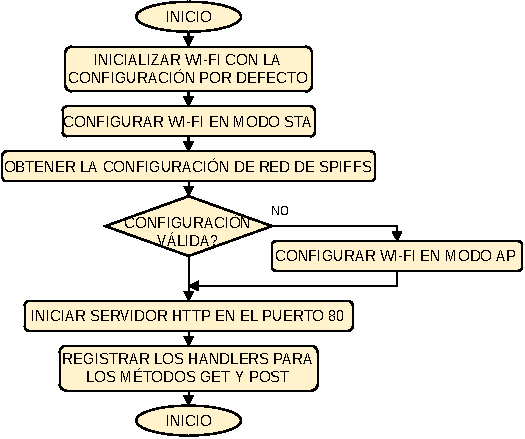
\includegraphics[scale=1]{./Figures/web_server_init.pdf}
	\caption{Diagrama de flujo de la función de inicialización del módulo WEB SERVER.}
		\label{fig:serverInit}
\end{figure}

En esta función el primer paso es inicializar la interfaz física de Wi-Fi con la configuración por defecto del ESP8266. Se configura el dispositivo en modo estación y se busca en el archivo config.txt configuración de red que permita conectarse a una red Wi-Fi existente. Si no existe dicha información o es inválida, se configura el dispositivo en modo punto de acceso. En cualquiera de los dos casos el siguiente paso es iniciar un servidor HTTP en el puerto 80 y finalmente registrar todos los handlers para los métodos GET y POST.

%----------------------------------------------------------------------------------------

\section{Interfaz web}

El diseño e implementación de una interfaz web tiene como objetivo proporcionar a los usuarios, es decir, a los abonados de las compañías eléctricas, la capacidad de interactuar con el dispositivo para visualizar gráficamente información relativa a su consumo eléctrico y configurar parámetros de la conexión Wi-Fi.

Para el desarrollo se utilizó el IDE Visual Studio Code, que ofrece un entorno de desarrollo muy intuitivo y también brinda la posibilidad de descargar \textit{plugins} que facilitan la escritura de código. Asimismo, se utilizaron distintos lenguajes enfocados en el desarrollo web, para brindar a la interfaz una estructura bien definida, estética y funcionalidad. Estos fueron:

\begin{itemize}
	\item HTML: se utilizó para definir todos los aspectos estructurales de la interfaz, como la ubicación de los elementos, las llamadas a bibliotecas externas y otros parámetros informativos. La versión utilizada fue HTML 5.
	\item CSS: brindó control sobre la presentación, formato y el diseño de la interfaz.
	\item JavaScript: permitió dotar de funcionalidad a los elementos de la interfaz. Fue necesaria para realizar el procesamiento de los datos provenientes del dispositivo.
	\item jQuery Mobile: con esta biblioteca fue posible darle a la interfaz un aspecto de aplicación para teléfonos móviles, además de la capacidad de adaptarse a cualquier tamaño de pantalla sin que la información mostrada se vea alterada.
	\item Highcharts: a través de esta biblioteca se logró exhibir la información de consumo eléctrico en un gráfico de barras, de esta manera es más comprensible para el usuario.\end{itemize}

La interfaz web está dividida en dos pantallas, principal y de configuración. La primera es meramente informativa y es donde se muestra el consumo eléctrico al usuario. La segunda permite conectar el dispositivo a un red Wi-Fi existente.

La pantalla principal fue diseñada pensando en brindarle al usuario la información de su consumo eléctrico de la manera más simple posible. En la mayor parte del área de la pantalla se muestra un gráfico de barras que presenta el consumo eléctrico de los últimos tres meses y en la esquina superior izquierda, un pequeño botón que dirige a la pantalla de configuración.

Al cargar la interfaz en un navegador web, se obtiene mediante el método GET el archivo pulses.csv que contiene los valores de consumo eléctrico que están almacenados en el dispositivo. Estos son procesados con instrucciones escritas en JavaScript para que la biblioteca Highcharts los utilice y genere el gráfico de barras. En la figura \ref{fig:interfaceMain} se observa la pantalla principal de la interfaz web.

\begin{figure}[h]
	\centering
	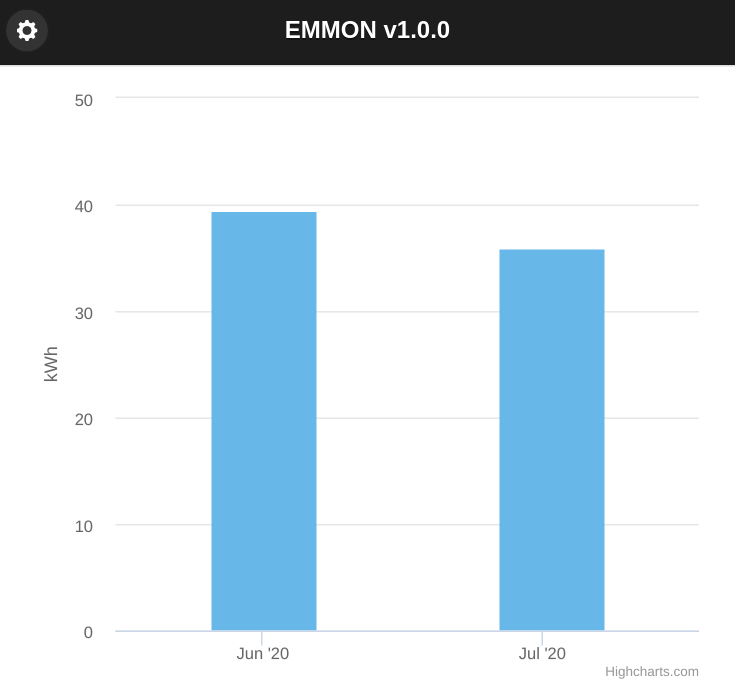
\includegraphics[scale=0.33]{./Figures/interface_main.png}
	\caption{Pantalla principal de la interfaz web.}
	\label{fig:interfaceMain}
\end{figure}

Se diseñó la pantalla de configuración para que la única configuración que puede realizarse sea la conexión del dispositivo a una red Wi-Fi existente a través de su SSID y contraseña. Esta pantalla es imprescindible, debido a que el dispositivo no debería ser manipulado manualmente bajo ninguna circunstancia por el usuario y se necesitaba una forma de realizar esta configuración.

El componente principal es un formulario para ingresar el SSID y la contraseña de la red a la que el usuario desea conectar el dispositivo. En la esquina superior izquierda se encuentra un botón para retornar a la pantalla principal y en la esquina superior derecha, un botón para enviar por el método POST el contenido del formulario al dispositivo. En la figura \ref{fig:interfaceConf} se muestra la pantalla de configuración de la interfaz web.

\begin{figure}[h]
	\centering
	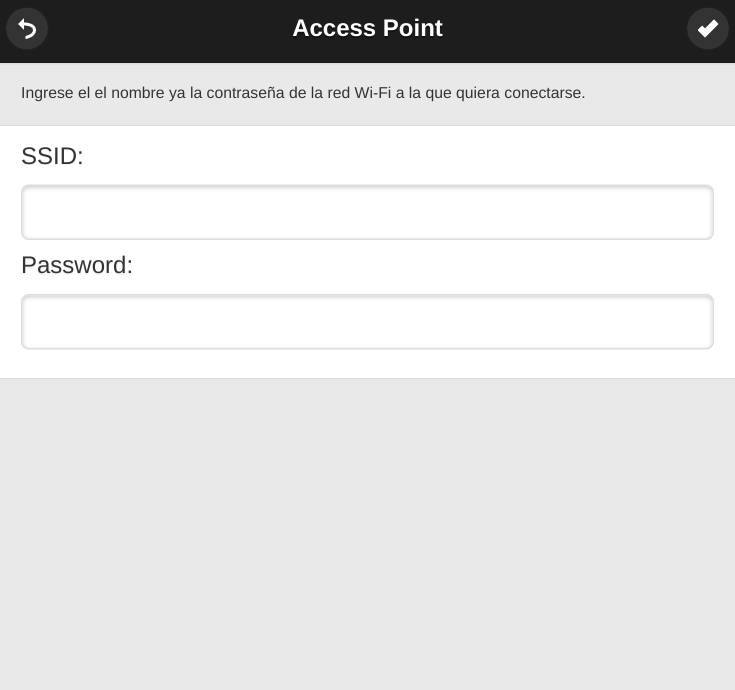
\includegraphics[scale=0.33]{./Figures/interface_conf.png}
	\caption{Pantalla de configuración de la interfaz web.}
	\label{fig:interfaceConf}
\end{figure}
%----------------------------------------------------------------------------------------

\section{Prototipo comercial}

El desarrollo de un prototipo para ser comercializado fue necesario para una primera implementación del dispositivo en un entorno real de trabajo y la realización de pruebas a nivel físico. Consta de una carcasa y un PCB (\textit{Printed Circuit Board}, tarjeta de circuito impreso).

El primer paso fue elegir una carcasa de dimensiones adecuadas para que pueda ser montada directamente sobre un medidor de consumo eléctrico domiciliario. Para este fin, se estudió la posibilidad de diseñar una carcasa personalizada, pero, debido a los altos costos de producción a nivel de prototipo, esta idea fue rápidamente descartada. Entonces, después de realizar un análisis de las dimensiones de los medidores utilizados por COPELECT, se eligió una carcasa disponible en el mercado internacional, la VG-S43 de la firma Vange. La elección de esta carcasa sobre otras similares, fue debido a los zócalos que tiene, que se adecuaban perfectamente para que el fototransistor estuviera descubierto y tuviera vista directa con el LED del medidor eléctrico. En la figura \ref{fig:case} se puede apreciar la carcasa elegida.

\begin{figure}[h]
	\centering
	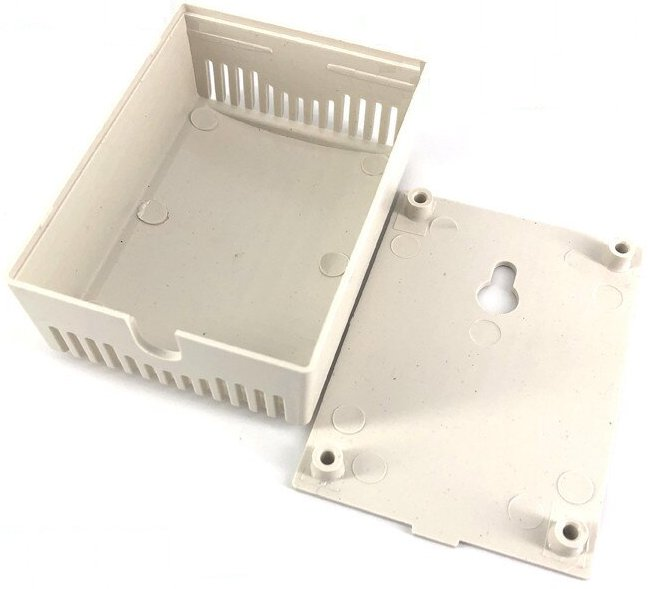
\includegraphics[scale=0.4]{./Figures/case.jpg}
	\caption{Carcasa VG-S43 de la firma Vange\protect\footnotemark.}
		\label{fig:case}
\end{figure}

	\footnotetext{Imagen tomada de: \url{https://es.aliexpress.com/item/33004284623.html?spm=a2g0o.cart.0.0.50483c00xuS0Xo&mp=1}}

Antes de empezar con el diseño del PCB, se realizó la elección de los componentes que serían parte del mismo. En el prototipo de pruebas se utilizaron módulos y tarjetas de desarrollo que con el firmware implementado en ellos, cumplieron todos los requerimientos planteados. Entonces, para que el firmware desarrollado pudiera ser utilizado exitosamente en el prototipo comercial, se utilizaron los circuitos integrados principales de los módulos y tarjetas de desarrollo, también se descartaron los componentes electrónicos que no resultaban necesarios para este trabajo. Existen dos componentes que se implementaron como módulos, el ESP-12S que es una variante del ESP-12F, componente principal de la NodeMCU, y el RA-01, que es un transceptor LoRa basado en el mismo circuito integrado que el PM1280, el SX1278. Además, el PT333-3C fue sustituido por el PT11-21C, que también es un fototransistor de similares características, pero es un SMD (\textit{Surface-Mount-Device}, dispositivo de montaje superficial).

Una vez elegidos los componentes implicados, se realizó un análisis del consumo de corriente de cada uno de ellos para implementar una fuente de alimentación adecuada. Cabe resaltar que la tensión de alimentación de todos los componentes es 3,3 V. En la tabla \ref{tab:componentsPower} se muestran los valores máximos de consumo de corriente de los componentes, estos datos fueron obtenidos de los respectivos datasheets.

\begin{table}[h]
	\centering
	\caption[Consumo de corriente del prototipo comercial]{Tabla de consumo de corriente eléctrica de los componentes del prototipo comercial.}
	\begin{tabular}{l c}    
		\toprule
		\textbf{Componente} & \textbf{Consumo de corriente (mA)} \\
		\midrule
		ESP-12S 	& 500 (en modo de transmisión continua) \\		
		RA-01		& 93 (en modo transmisor)\\
		DS3231		& 0,2 (en modo activo) \\
		AT24C32 	& 3 (cuando se escribe un dato)\\
		LM393 		& 20 (cortocircuitado a tierra) \\
		PT11-21C	& 20 \\
		\bottomrule
		\hline
	\end{tabular}
	\label{tab:componentsPower}
\end{table}

De la tabla \ref{tab:componentsPower}, se determinó que el consumo total de todos los componentes es de 636,2 mA. Al momento de elegir la fuente de alimentación al consumo total se le añadió un margen de seguridad del 50\%, que dio un nuevo valor de 954,43 mA. Por lo tanto, la fuente de alimentación elegida debió ser de 3.3 V y 1 A.

Para reducir la cantidad de componentes de la fuente de alimentación, se escogió un módulo conversor de energía alterna a directa. De esta forma, el prototipo comercial podría conectarse directamente a la misma línea eléctrica del medidor. El componente elegido fue el módulo HLK-PM03 de la firma Hi-Link, que proporciona 3,3 V y 1 A a su salida, cuando a la entrada existen 90 V - 240 V alternos. En la figura \ref{fig:powerModule} puede observarse el módulo para la fuente de alimentación.

\begin{figure}[h]
	\centering
	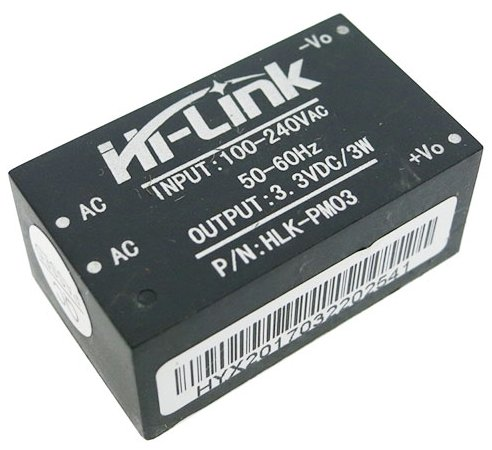
\includegraphics[scale=0.26]{./Figures/acdc_module.jpg}
	\caption{Módulo de alimentación HLK-PM03 de la firma Hi-Link\protect\footnotemark.}
		\label{fig:powerModule}
\end{figure}

	\footnotetext{Imagen tomada de: \url{https://es.aliexpress.com/item/33004284623.html?spm=a2g0o.cart.0.0.50483c00xuS0Xo&mp=1}}
	
Con ayuda del software KiCAD, se realizó el dibujo de un diagrama esquemático del prototipo comercial, que interconecta todos los componentes y brinda información relacionada a aspectos importantes sobre el funcionamiento y diseño del PCB. En la figura \ref{fig:schematic} se muestra el diagrama esquemático del prototipo comercial.

\begin{figure}[h]
	\centering
	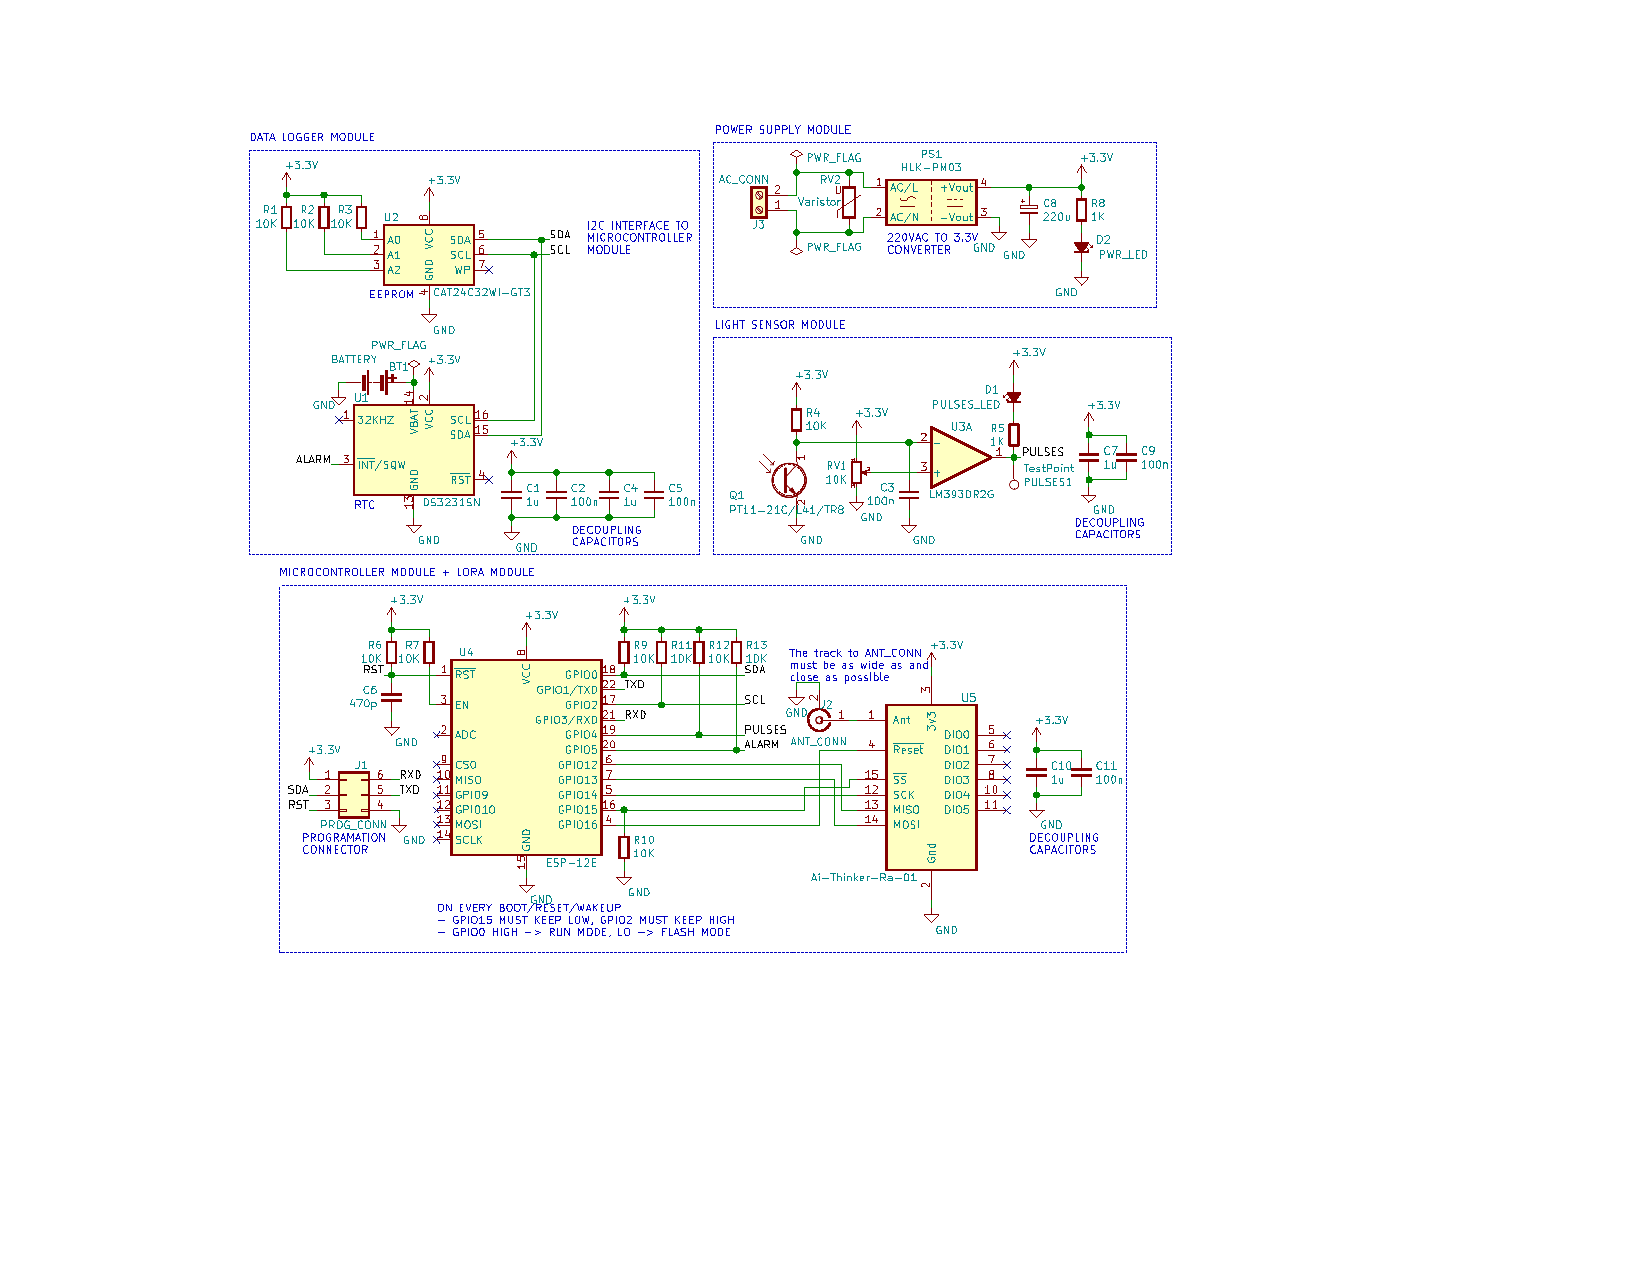
\includegraphics[scale=0.9]{./Figures/schematic.pdf}
	\caption{Diagrama esquemático del prototipo comercial.}
		\label{fig:schematic}
\end{figure}

Del diagrama anterior, se puede notar que se añadieron \textit{test points} para poder probar la respuesta del sensor de luz mediante instrumentación especializada. Se añadieron también un conector destinado a la depuración del código almacenado en el ESP8266, junto con LEDs para monitorear el estado de la fuente y el sensor de luz.

Con el diagrama esquemático finalizado, se realizó la ERC (\textit{Electrical Rule Check}, comprobación de reglas eléctricas) en busca de posibles cortocircuitos, conexiones ilegales y contactos flotantes entre otras comprobaciones. Posteriormente, se dibujó el circuito impreso, donde se tuvieron en consideración las restricciones físicas impuestas por la elección de la carcasa. Se hizo especial énfasis en la ubicación de los conectores, para que quedaran al borde del PCB y pudieran ser accedidos con mayor facilidad. El fototransistor quedó ubicado en una posición tal que coincidiera con el zócalo inferior de la carcasa. Otra consideración de importancia fue la distancia entre el transceptor LoRa y el conector coaxial, ambos componentes fueron ubicados muy cerca, de tal forma que la pista que los conectaba tuviera una distancia muy corta. Asimismo, se dibujó la pista lo más ancha posible y se pusieron vías conectadas a tierra para lograr una mejor respuesta a las interferencias electromagnéticas.

Las capas \textit{top} y \textit{bottom} del PCB, pueden apreciarse en las figuras \ref{fig:pcbTop} y \ref{fig:pcbBot}, respectivamente. Por otro parte, en las figuras \ref{fig:pcb3D} y \ref{fig:pcbReal}, se muestran el modelo 3D renderizado del PCB y una fotografía del PCB montado.

\begin{figure}[h]
	\centering
	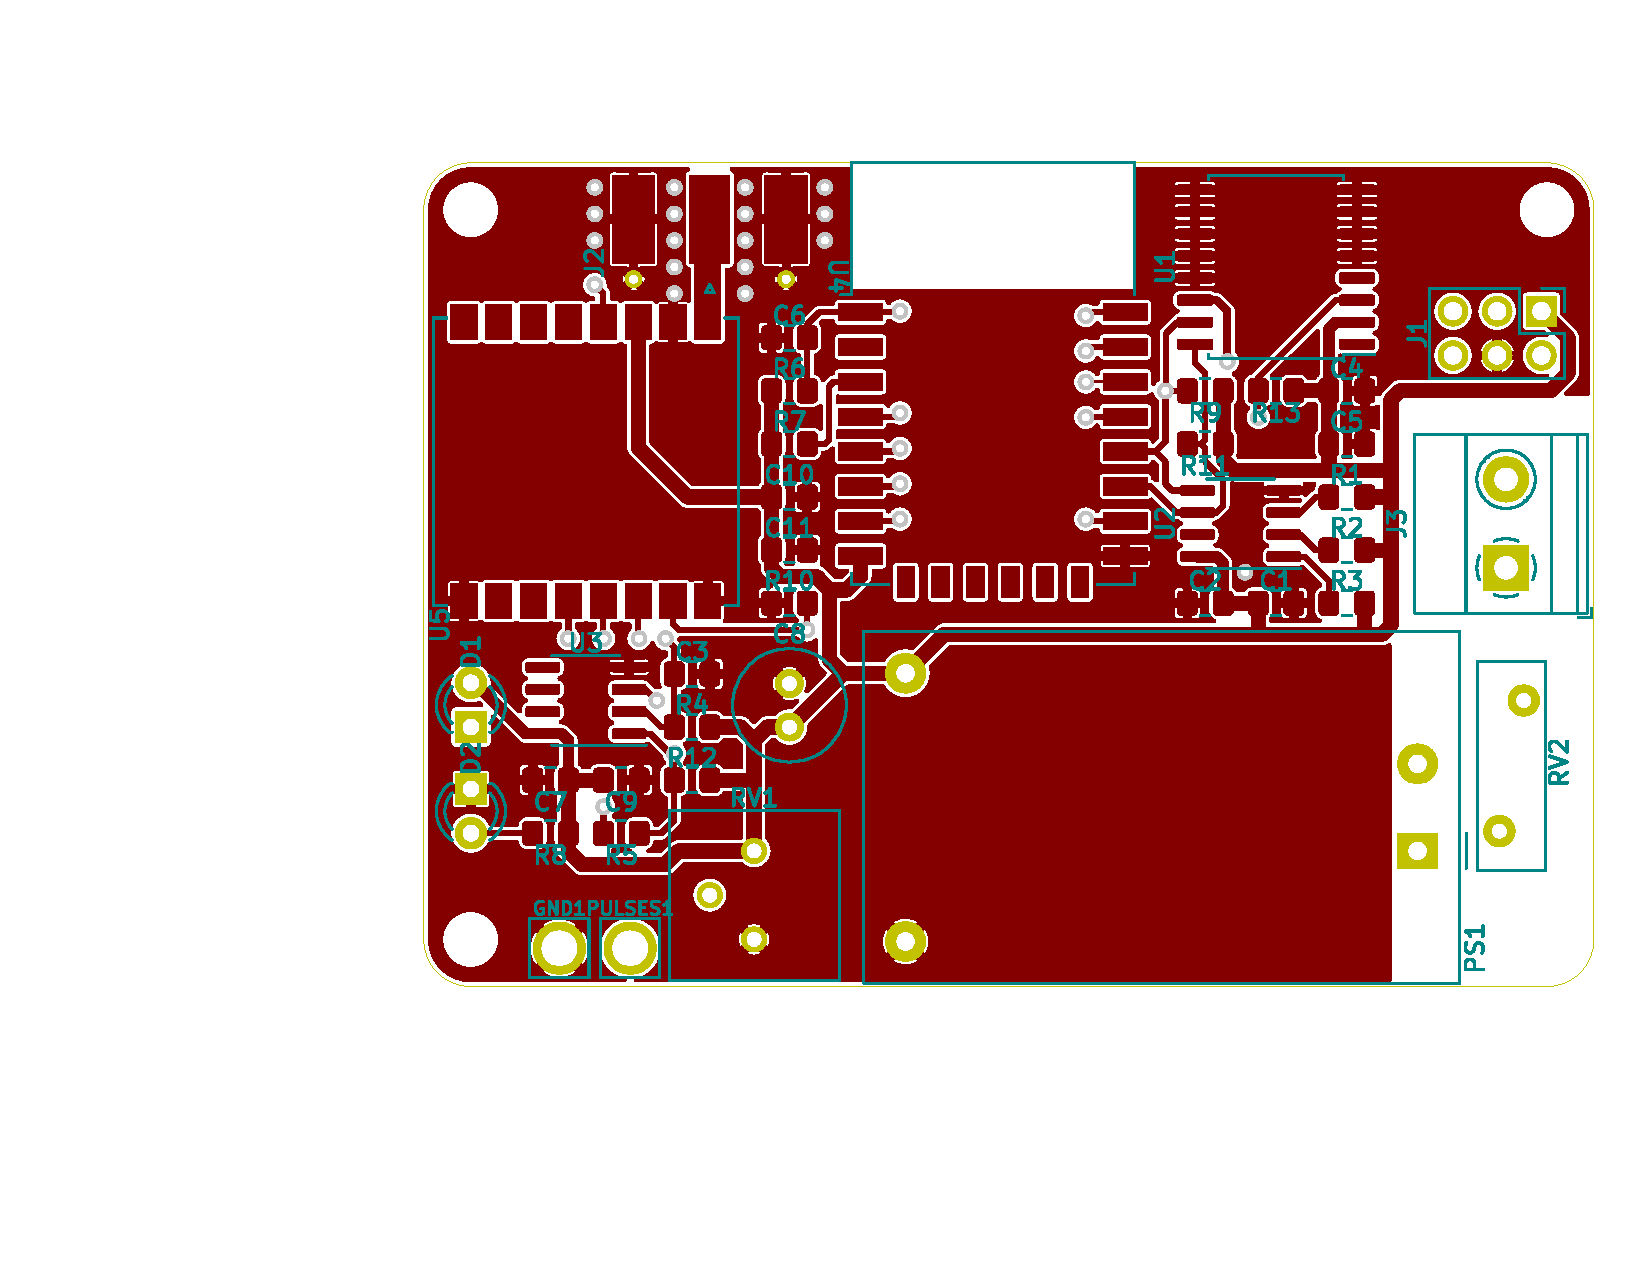
\includegraphics[scale=0.5]{./Figures/pcb_top.pdf}
	\caption{Capa top del PCB.}
		\label{fig:pcbTop}
\end{figure}

\begin{figure}[h]
	\centering
	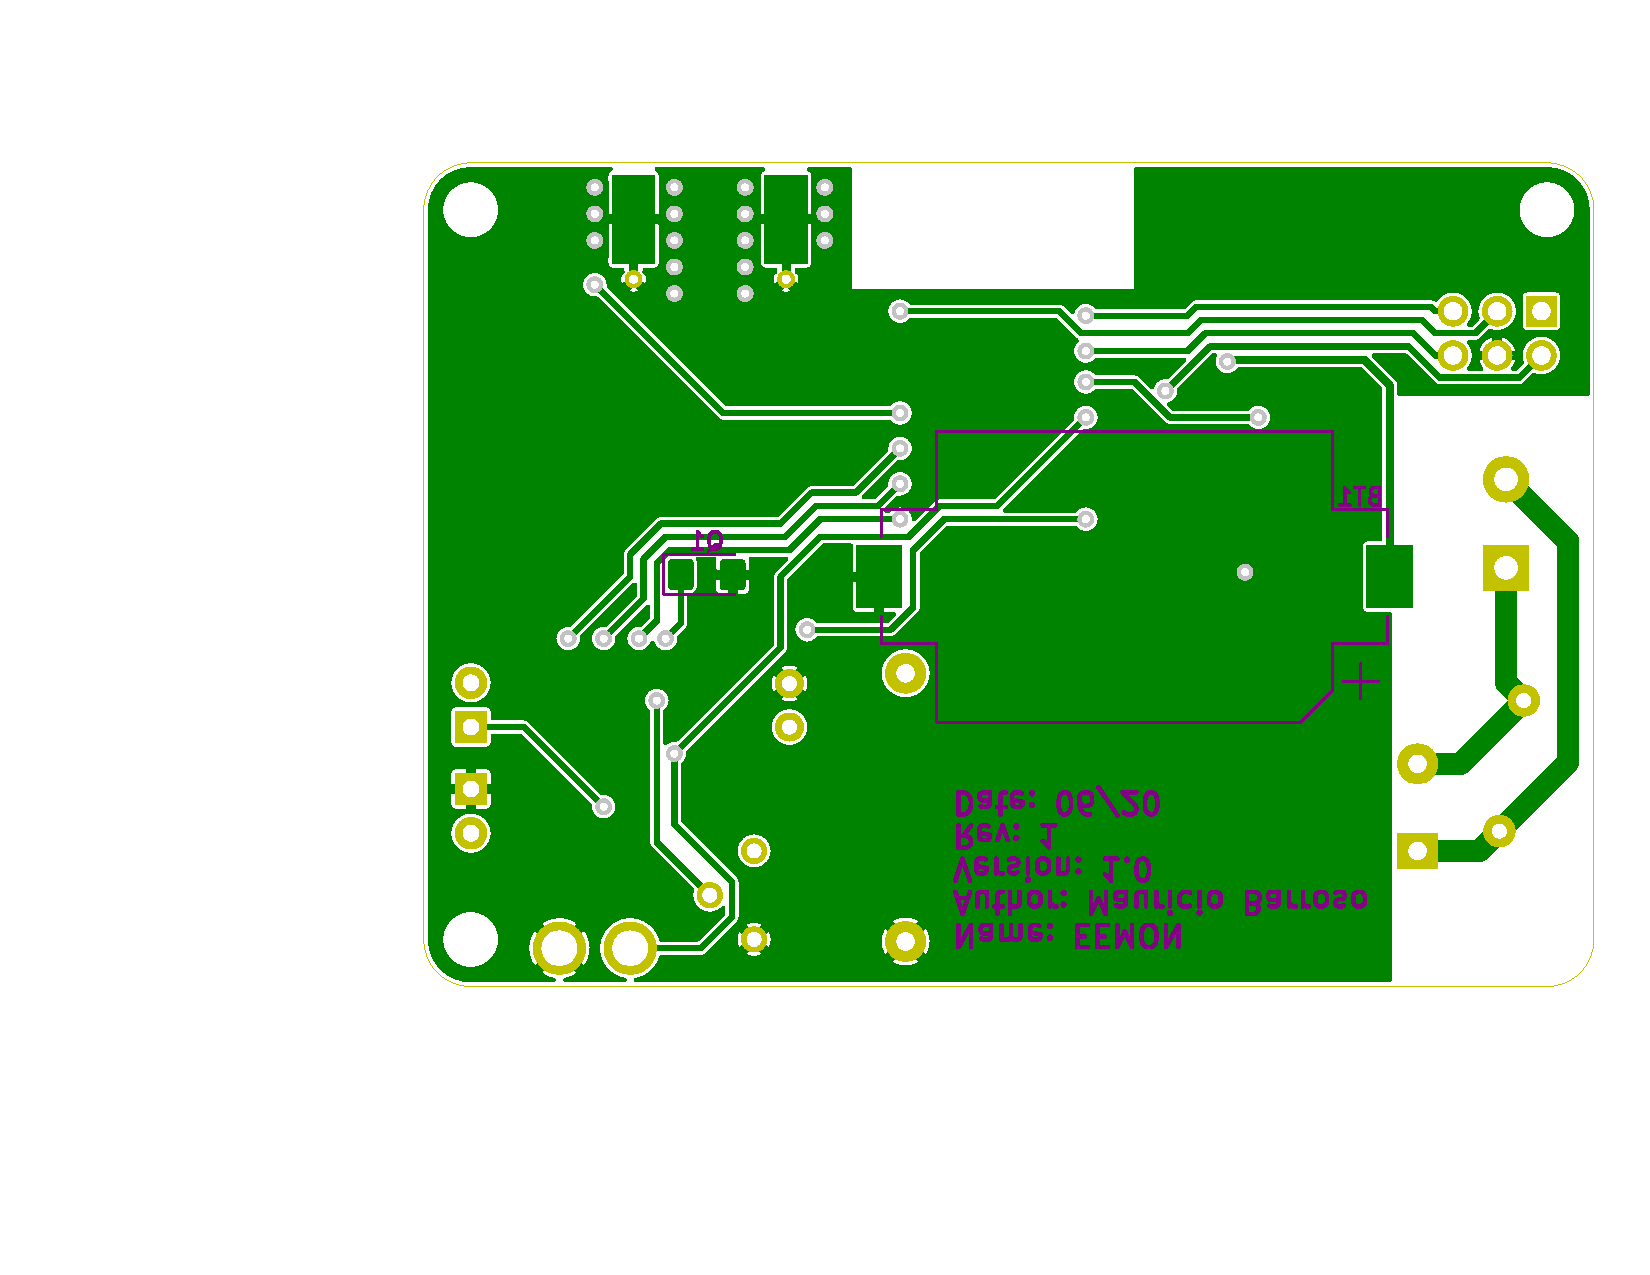
\includegraphics[scale=0.5]{./Figures/pcb_bot.pdf}
	\caption{Capa bottom del PCB.}
		\label{fig:pcbBot}
\end{figure}

\begin{figure}[h]
	\centering
	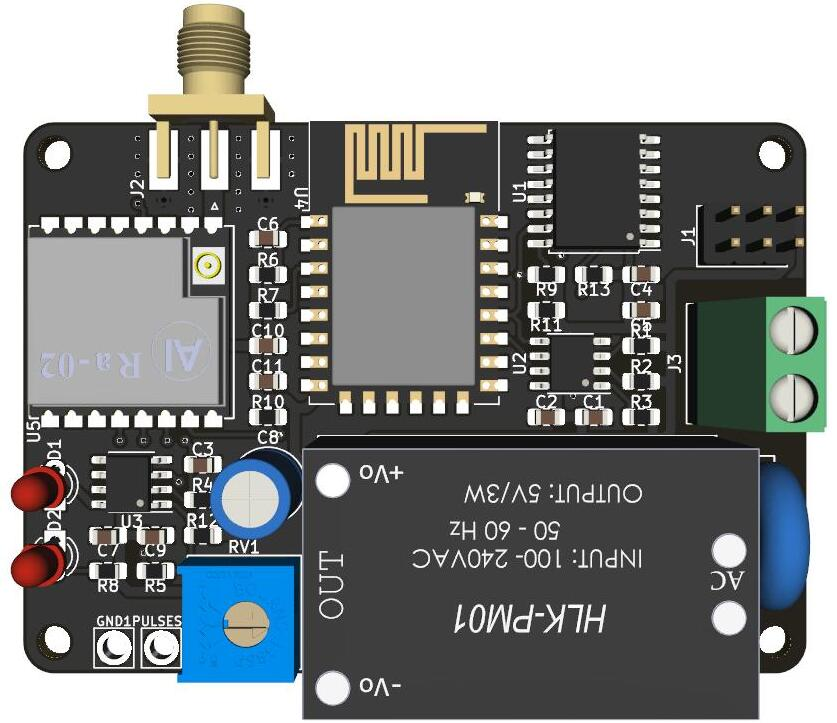
\includegraphics[scale=0.375	]{./Figures/pcb_3d.jpg}
	\caption{Modelo 3D del PCB montado del prototipo comercial.}
		\label{fig:pcb3D}
\end{figure}

\begin{figure}[h]
	\centering
	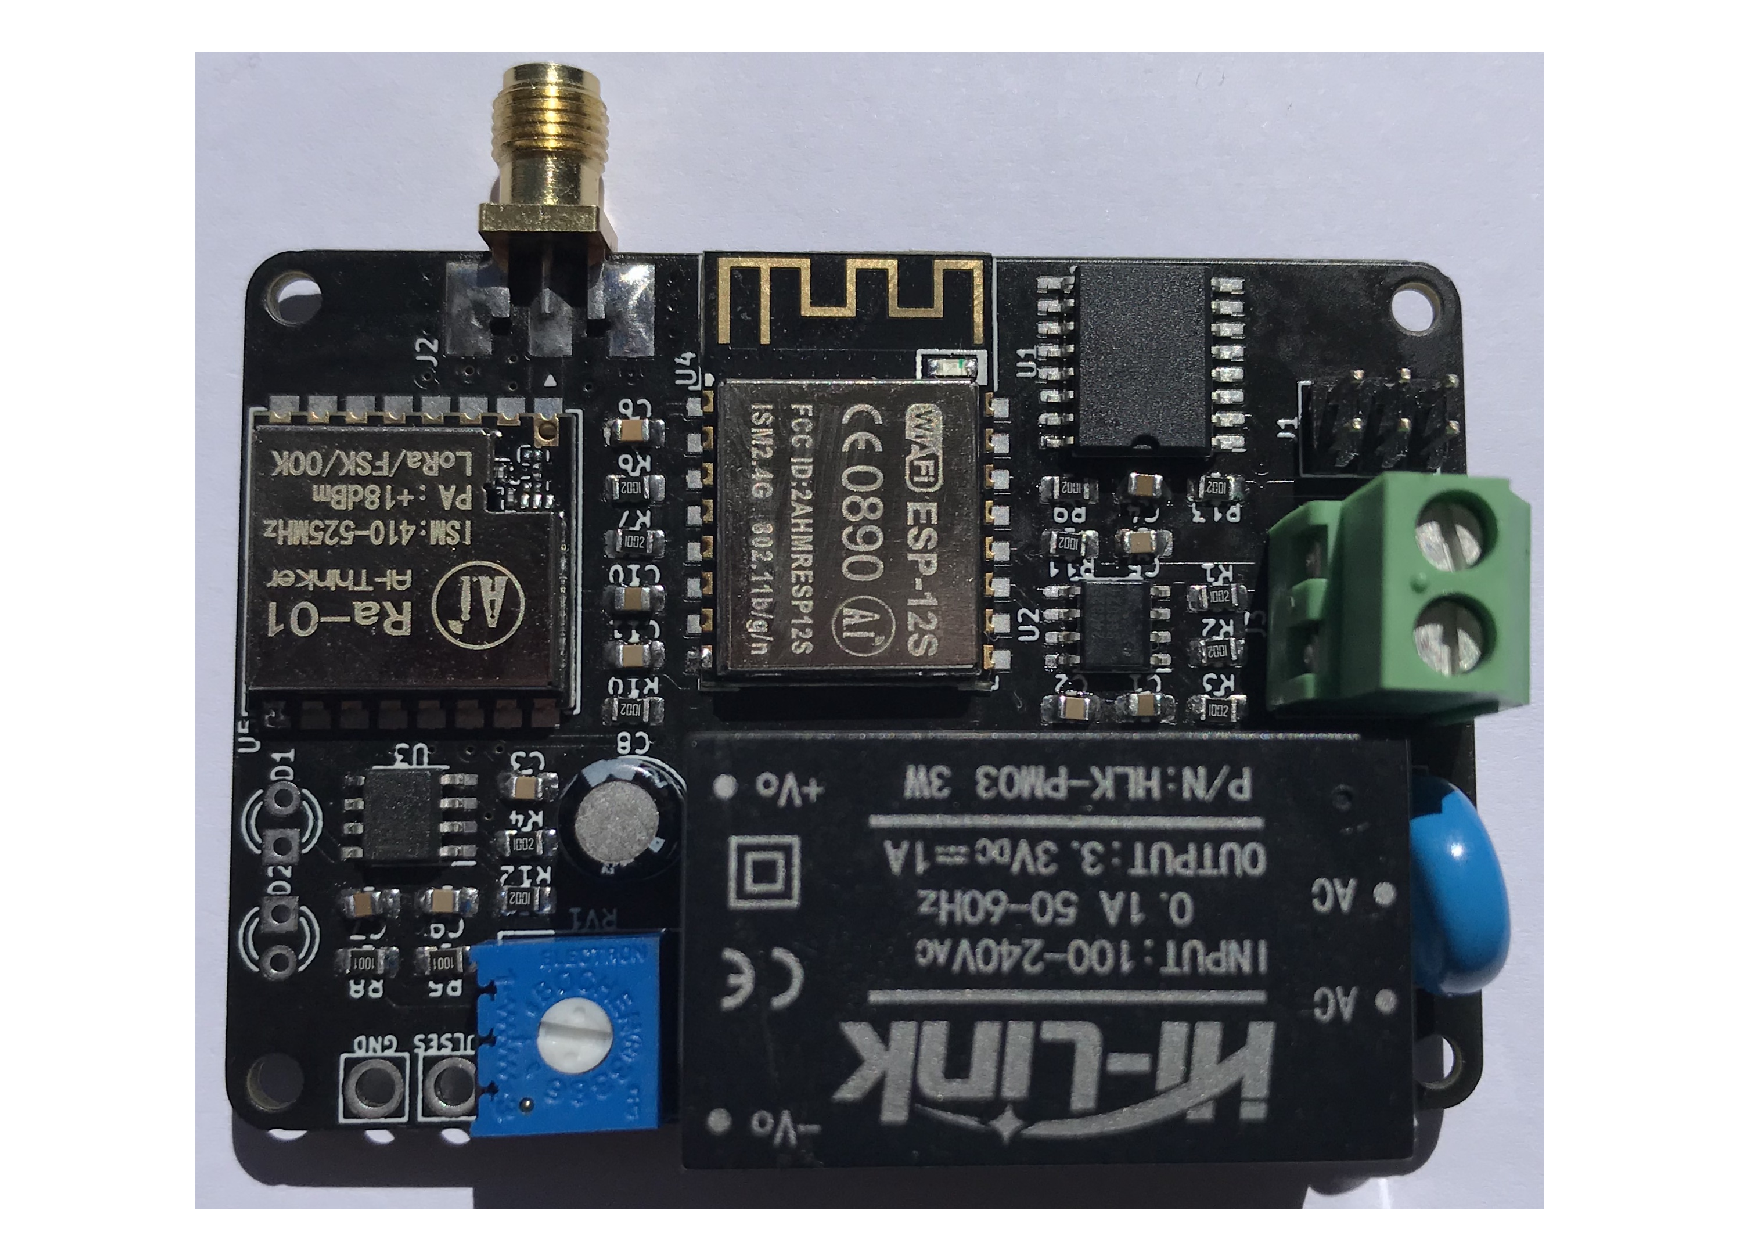
\includegraphics[scale=0.5	]{./Figures/pcb_real.pdf}
	\caption{PCB montado del prototipo comercial.}
		\label{fig:pcbReal}
\end{figure}

La manufactura del PCB fue realizada por el fabricante JLCPCB y los componentes fueron adquiridos de la firma LCSC. Ambos fueron elegidos por los costos reducidos que ofrecen en sus productos, además de que JLCPCB ofrece el servicio de PCBA (\textit{Printed Circuit Board Assembly}, montaje de PCB) con los componentes que tiene disponibles LCSC.